\documentclass[10pt]{beamer}
%\documentclass[10pt,handout]{beamer}
\usepackage[spanish]{babel}
% % \usepackage[backend=biber, style=authoryear-icomp]{biblatex}
\resetcounteronoverlays{exx}
\usepackage{mdframed}
\usepackage{tikz}
\usepackage{blindtext}
\usepackage{tipa}
% \usepackage{cgloss4e}
% \usepackage{gb4e}
% \usepackage{qtree}
\usepackage{cancel}
\usepackage{wrapfig}
\usepackage{soul}
\usepackage{enumerate}
\usepackage{longtable}
\graphicspath{ {../img/} } % declaramos donde estan las imagenes
\usepackage[labelformat=simple]{subcaption} % para varias imagenes juntas
\renewcommand\thesubfigure{(\alph{subfigure})}
\usepackage[utf8]{inputenc}
\usepackage{amsmath}
\usepackage{amsfonts} % simbolos como el I de matriz identidad
\usepackage{bm}
\usepackage{graphicx} % paquete para ver imagenes
\usepackage{setspace}
\usepackage[T1]{fontenc}
\usepackage{parskip}
\usepackage{color}
\usepackage{framed}
\usetheme{Copenhagen}
\definecolor{frenchblue}{rgb}{0.0, 0.45, 0.73} % ESTE!!!!
\definecolor{myblue1}{RGB}{35,119,189}
\definecolor{myblue2}{RGB}{95,179,238}
\definecolor{myblue3}{RGB}{129,168,207}
\definecolor{myblue4}{RGB}{26,89,142}

\setbeamercolor{block body}{bg=frenchblue!50}
\setbeamercolor*{structure}{fg=frenchblue,bg=blue}
\setbeamertemplate{frametitle}[default][center]
\setlength{\parskip}{12pt}
\useoutertheme{infolines} % me comia mucho espacio de la otra fgorma
\makeatother
\setbeamertemplate{footline}
{
  \leavevmode%
  \hbox{%
  \begin{beamercolorbox}[wd=.3\paperwidth,ht=2.25ex,dp=1ex,center]{author in head/foot}%
    \usebeamerfont{author in head/foot}\insertshortauthor
  \end{beamercolorbox}%
  \begin{beamercolorbox}[wd=.6\paperwidth,ht=2.25ex,dp=1ex,center]{title in head/foot}%
    \usebeamerfont{title in head/foot}\insertshorttitle
  \end{beamercolorbox}%
  \begin{beamercolorbox}[wd=.1\paperwidth,ht=2.25ex,dp=1ex,center]{date in head/foot}%
    \insertframenumber{} / \inserttotalframenumber\hspace*{1ex}
  \end{beamercolorbox}}%
  \vskip0pt%
}
\newcommand{\floor}[1]{\lfloor #1 \rfloor}

\makeatletter
\setbeamertemplate{navigation symbols}{}
%\setbeameroption{show notes}
\setbeameroption{hide notes}


\usepackage{hyperref}

\title[Reporte quincenal]{Reporte quincenal}
\author[Matias Mazzanti]{Matias Mazzanti}


\begin{document}


\section{Organización}
%%%%%%%%%%%%%%%%%%%%%%%%%%%%%%%%%%%%%%%%%%%%%%%%%%%%%%%%%%%%%%%%%%%%%%%%%%%%%%%%%%%%%%%%%%%%%%%%%%%%

\begin{frame}
\frametitle{OpenFHE-''avances''}

Compilar sin OpenMP - single thread.
\vspace{-0.6cm}
\begin{figure}[h!]
    \centering
    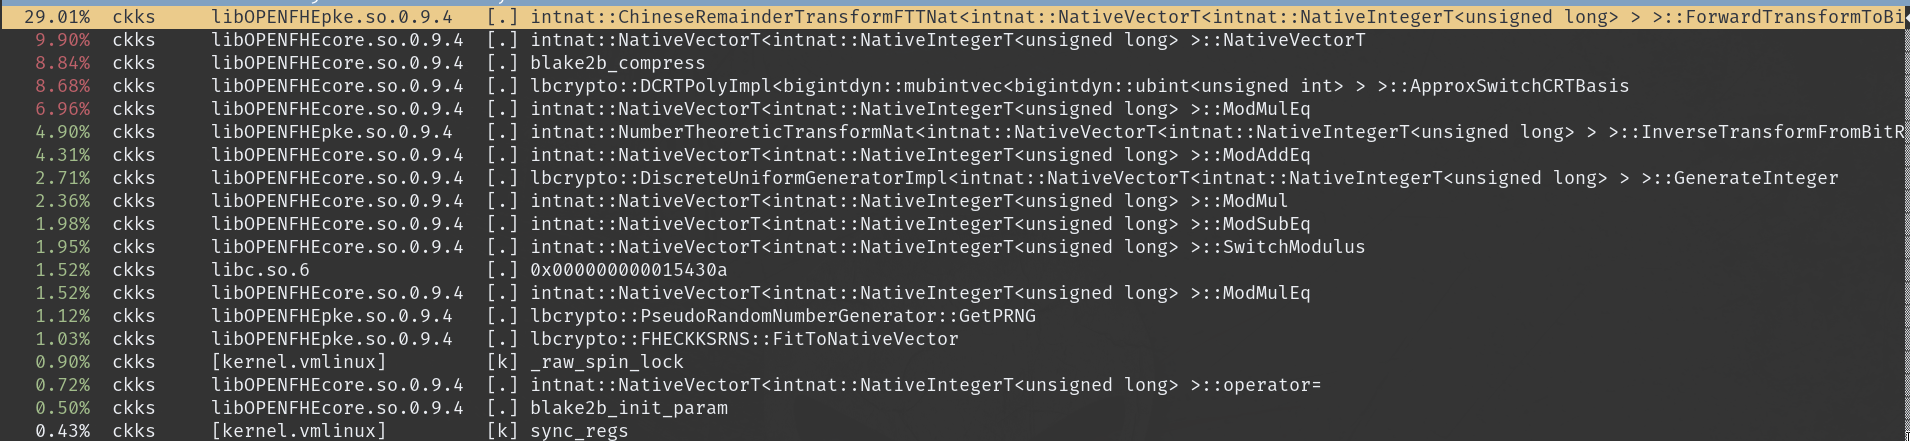
\includegraphics[scale=0.18]{perf.png}
\end{figure}
\pause

\vspace{-0.3cm}
Compilar ejemplo sin cmake complejo.

Visualizador de perf: hotspot y flamegraph (sin probar todavía)

\pause
Entender ''mejor'' CKKS, codificación y decodificación.

\pause
(Avances de curso Onur y programación en C no los considero.)
\end{frame}
%%%%%%%%%%%%%%%%%%%%%%%%%%%%%%%%%%%%%%%%%%%%%%%%%%%%%%%%%%%%%%%%%%%%%%%%%%%%%%%%%%%%%%%%%%%%%%%%%%%%

\begin{frame}
\frametitle{CKKS}
\begin{figure}[h!]
    \centering
    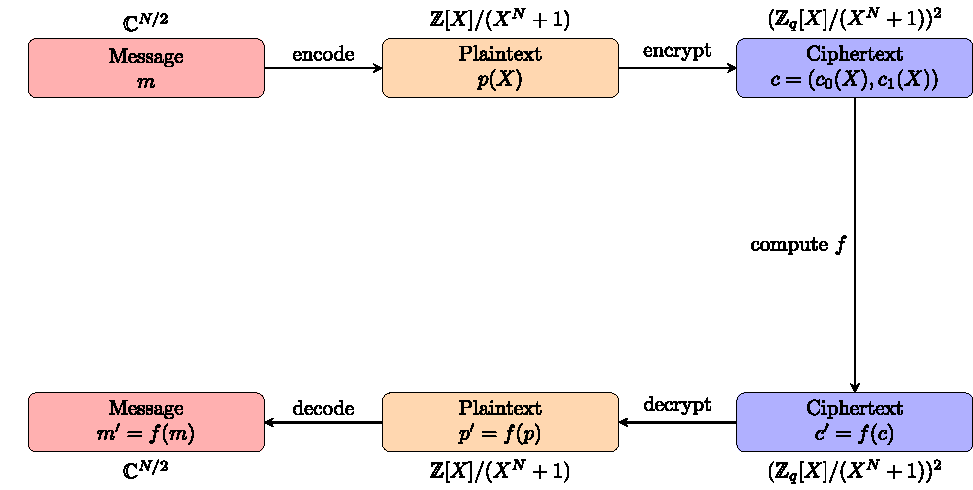
\includegraphics[scale=0.6]{Cryptotree_diagrams-2.pdf}
\end{figure}


\end{frame}


%%%%%%%%%%%%%%%%%%%%%%%%%%%%%%%%%%%%%%%%%%%%%%%%%%%%%%%%%%%%%%%%%%%%%%%%%%%%%%%%%%%%%%%%%%%%%%%%%%%%

\section{Lo siguiente}
\begin{frame}
\frametitle{CKKS encoder/decoder}

CKKS usa las estructuras de anillos de polinomios enteros.

Sea $z\in \mathbb{C}^{N/2}$, codificarlo en un polinomio  $m(X)\in \mathcal{R} = \mathbb{Z}[X]/(X^N+1)$

Con modulo $N$, múltiplo de 2.

\pause
Se define $M=2N$.

Se usa el \textbf{encaje canónico} (\texttt{canonical embeddign}) $\sigma$:
nos da isomorfismo, entre vectores y polinomios.

\pause

En particular, el m-esimo \textbf{polinomio cíclico} $\Phi_M(X)= X^N+1$.


Sus \textbf{raíces} de la unidad: $\xi_M=(e^{2i\pi/M})^k$, $k\in \mathbb{Z}<M$ y coprimos de $M$.


\end{frame}


%%%%%%%%%%%%%%%%%%%%%%%%%%%%%%%%%%%%%%%%%%%%%%%%%%%%%%%%%%%%%%%%%%%%%%%%%%%%%%%%%%%%%%%%%%%%%%%%%%%%
\begin{frame}
\frametitle{CKKS encoder/decoder simplificado}

La decodificación es sencilla.

Dado $m(X)$, se evalua el polinomio en las raices.

\pause
Es decir $\sigma(m) = (m(\xi), m(\xi^3),..., m(\xi^{2N-1}))= (z_1, z_2, ..., z_N)$. Más algunos detalles (en breve).

\textbf{Complejidad}: como calcular $\sigma^{-1}$. Como codificar el vector $z$.

\pause
La forma ''facil'': $\sigma: \mathbb{C}[X]/(X^N+1) \to \mathbb{C}^N$

$m(X) = \sum_{j=0}^{N-1} \alpha_j X^j$ $\to$ $z_j =  \sum_{j=0}^{N-1} \alpha_j (\xi^{2i-1})^j$

\pause
Sistema lineal $A\alpha=z$ con $A$ una matriz de Vandermonde de $\xi^{2j-1}$, $\alpha$ vector
de los coeficientes del polinomio.

Entonces: $\alpha = A^{-1}z \to \sigma^{-1}(z)=\sum_{j=0}^{N-1} \alpha_j X^j$
\end{frame}

%%%%%%%%%%%%%%%%%%%%%%%%%%%%%%%%%%%%%%%%%%%%%%%%%%%%%%%%%%%%%%%%%%%%%%%%%%%%%%%%%%%%%%%%%%%%%%%%%%%%
\begin{frame}
\frametitle{CKKS encoder}

Resolvimos  esto al revés $ \mathbb{C}^N \to \mathbb{C}[X]/(X^N+1)$ queremos
$ \mathbb{C}^{N/2} \to \mathcal{R} =\mathbb{Z}[X]/(X^N+1)$.

Es decir $m(X)$ tiene que tener coeficientes enteros.

\pause
Con esto, al evaluarlo con raíces complejas, donde la mitad de estas son complejas
conjugadas de las otras, tenemos:

$\sigma(\mathcal{R}) \to z_j=\overline{z_{-j}} \to m(\xi^j)=m(\overline{\xi^{-j}})$.

\pause
Entonces usamos vectores $z\in\mathbb{C}^{N/2}$ y lo extendemos con sus conjungados (paper $\pi^{-1}$).

\pause
Para mantener el isomorfismo de $\sigma(\mathcal{R})\to \mathcal{R}$ (recordemos que están
en diferentes espacios ahora) tenemos que proyectar $\pi^{-1}$ a $\sigma(\mathcal{R})$ de
alguna forma.
\end{frame}

%%%%%%%%%%%%%%%%%%%%%%%%%%%%%%%%%%%%%%%%%%%%%%%%%%%%%%%%%%%%%%%%%%%%%%%%%%%%%%%%%%%%%%%%%%%%%%%%%%%%
\begin{frame}
\frametitle{CKKS encoder}

Como $\mathcal{R}$ tiene una base $\mathbb{Z}$ ortogonal $1, X,...,X^{N-1}$ y que $\sigma$ es
un isomorfismo, entonces $\sigma(\mathcal{R})$ también tiene una.

Sea $\beta = (b_1,...,b_N)=(\sigma(1),\sigma(X),...,\sigma(X^{N-1}))$.

\pause
Entonces para cualquier $Z=\pi^{-1}(z)\in \mathbb{C}^N$ (rec:$z\in\mathbb{C}^{N/2}$ )
lo proyecto en $\beta$.

\begin{equation*}
Z=\sum_{i=1}^N\frac{<Z,b_i>}{|| b_i||^2}b_i
\end{equation*}

\pause

Por ultimo usamos el algoritmo de \texttt{coordinate-wise random rounding} para
redondear los $Z_i$ reales en enteros.
(Redondea x a $\floor{x}$ o $\floor{x}+1$ dando más proba mientras x este más cerca de alguno.)


Tendremos un polinomio $m\in \sigma(\mathcal{R})$, ya que tiene coeficientes enteros en la base $\beta$.

\end{frame}

%%%%%%%%%%%%%%%%%%%%%%%%%%%%%%%%%%%%%%%%%%%%%%%%%%%%%%%%%%%%%%%%%%%%%%%%%%%%%%%%%%%%%%%%%%%%%%%%%%%%
\begin{frame}
\frametitle{CKKS encoder}

Con esto simplemente aplicamos $\sigma^{-1}$ que nos dará la codificación
(un elemento de $\mathcal{R}$).

Como último detalle, para evitar que el redondeo elimine algunos números significativos,
se multiplica a $z$ por un factor $\bigtriangleup>0$ al principio de la codificación.

\pause
Para decodificar simplemente se divide por el mismo factor.


Es decir para codificar simplemente del texto plano $m(X)$ obtenemos
$z=\pi \circ \sigma(\bigtriangleup^{-1}.m)$

\end{frame}


\begin{frame}
\frametitle{Próxima reunion (propuesta)}

\begin{itemize}
  \item Cerrar algunas ideas de la codificación.
  \item Comparar implementación codificación OpenFHE con lo explicado hoy.
\pause
  \item Avanzar con encriptación de CKKS.
  \item Visualizador perf: navegar dentro del código.
\end{itemize}

\end{frame}
\end{document}

